\section*{Question 1:}
Exercise 10.3: 
Compute five iterations of HITS (see Algorithm 3) and PageRank (see Figure 4.11) on the graph in Figure 10.3. Discuss how the PageRank scores compare to the hub and authority scores produced by HITS

\subsection*{Answer:}

The graph below was copied from the textbook Figure 10.3. 


\begin{figure}[h]
\caption{Copied from the textbook Figure 10.3}
\centering
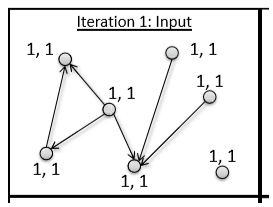
\includegraphics[scale=0.6]{Q1/hp.png}
\end{figure}

I used the same node numbers in the textbook. The graph below was copied from the textbook Figure 10.4.

\begin{figure}[h]
\caption{Copied from the textbook Figure 10.3}
\centering
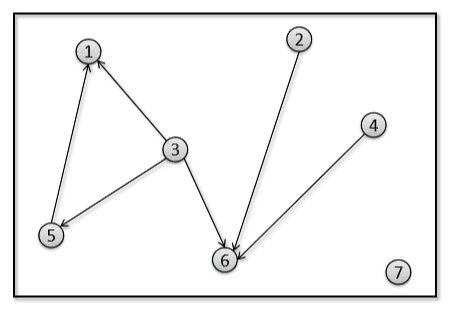
\includegraphics[scale=0.6]{Q1/hp1.png}
\end{figure}


I wrote a python script and named it hp.py to calculate HITS and PageRank scores using Link Analysis.


\lstinputlisting[language=python, label=hp.py, caption=The content of hp.py, breakatwhitespace=〈false)]{Q1/hp.py}


\textbf{Results}


